\documentclass{article}
%
% Demo of the mcode package from 
% http://www.mathworks.co.uk/matlabcentral/fileexchange/8015-m-code-latex-package
% Updated 06 Mar 2014
%

% load package with ``framed'' and ``numbered'' option.
\usepackage[framed,numbered,autolinebreaks,useliterate]{mcode}

% something NOT relevant to the usage of the package.
\usepackage{url}
\usepackage{graphicx}
\usepackage{subfigure}

\setlength{\parindent}{0pt}
\setlength{\parskip}{18pt}
\title{\texttt{Sistemas de Control Inteligente \newline} Práctica 1. Identificación y control neuronal (III)}
\author{Pablo Acereda García y Laura Pérez Medeiro}
% //////////////////////////////////////////////////

\begin{document}

\maketitle

\section{Identificación de un sistema usando una red NARX}

Usando el archivo proporcionado en la práctica, se crea un modelo usando ese sistema con una entrada aleatoria y almacenando las variables x e y en estructuras con tiempo, las cuales deben ser accesibles desde el Workspace. Para ello, se realizaran las siguientes configuraciones:


\begin{figure}[h]
\caption{Configuración para la entrada aleatoria}
\centering
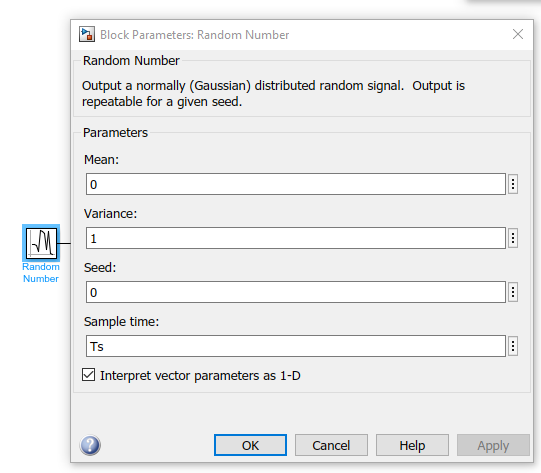
\includegraphics[width=0.5\textwidth]{imagenes/randomNumConf.png}
\end{figure}

\begin{figure}[h]
\caption{Configuración para la variable X, para que aparezca sin el formato out.X}
\centering
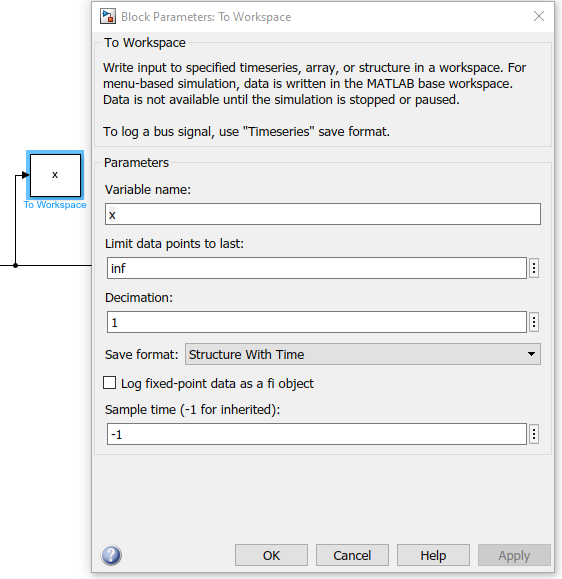
\includegraphics[width=0.5\textwidth]{imagenes/VarX.png}
\end{figure}

\begin{figure}[h]
\caption{Configuración para mostrar la variable en el área de trabajo de Matlab}
\centering
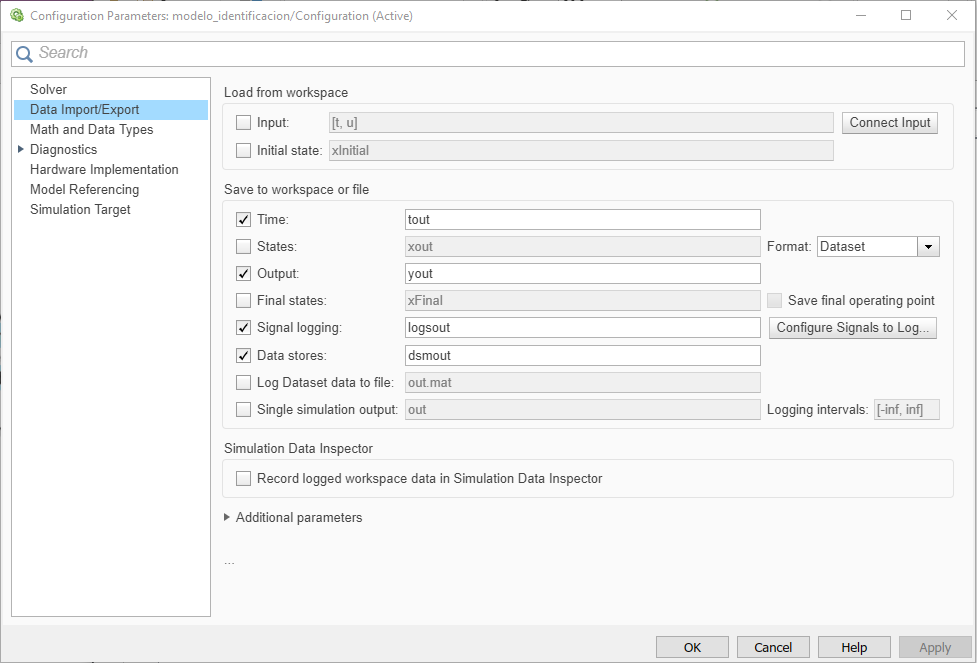
\includegraphics[width=0.5\textwidth]{imagenes/ConfigOut.png}
\end{figure}
\newpage
Mediante el siguiente código, el cual se encuentra en el archivo SimData.m, se generan los arrays de inputs y outputs:
\lstinputlisting{./Source/SimData.m}

A continuación se generará una red de tipo NARX con 5 neuronas en la capa oculta y dos retardos tanto en la entrada como la salida realimentada:
\lstinputlisting{./Source/NARX_NeuronalNetwork_1.m}

Comporbaremos el error de entreamiento de la red en los diferentes conjuntos de datos (test, validaton y train), mediante la gráfica plotperform, la cual se encuentra disponible en el menú de entrenamiento de la red:



\begin{figure}
    \begin{sufigure}
        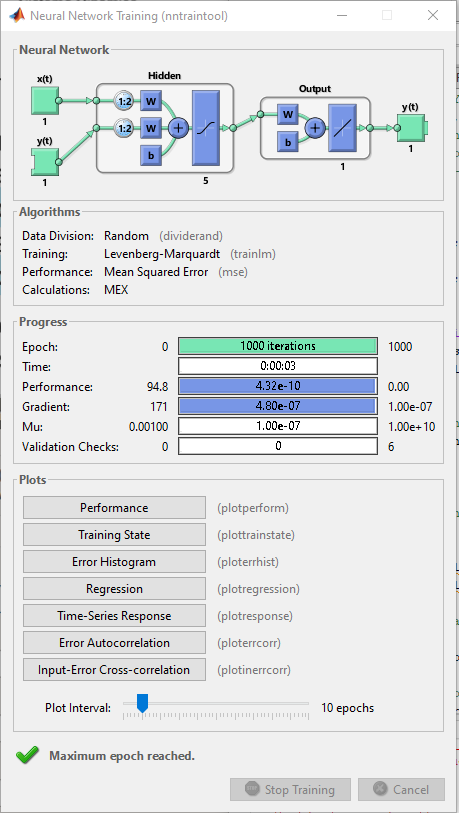
\includegraphics[width=0.25\textwidth]{imagenes/EX1_VIEWTRAIN.png}
    \end{sufigure}
    \begin{sufigure}
        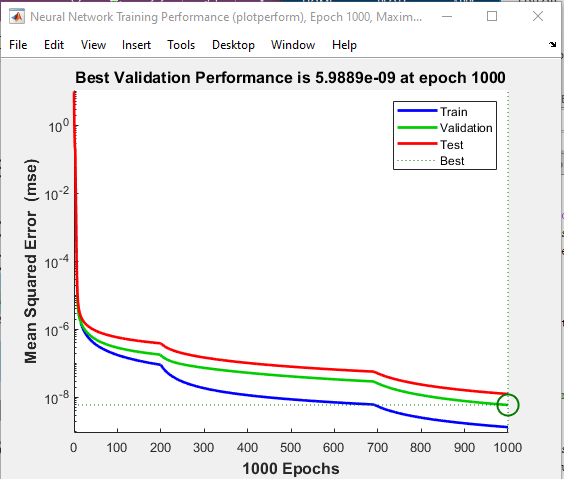
\includegraphics[width=0.5\textwidth]{imagenes/EX1_PERFORMANCE.png}
    \end{sufigure}
\end{figure}

\newpage
Finalmente, se genera un modelo de Simulink que contenga a la red entrenada mediante el comando: \mcode{gensim(net, Ts)}

\section{Seguimiento de la trayectoria mediante redes recurrentes}

\subsection*{Implementación del diagrama de control para seguimiento de trayectorias}

Para ello, se realizarán las mismas configuraciones aplicadas anteriormente. La única diferencia, se hata en la configuración de los integradores, donde la condición inicial dependerá de las variables x\_0, y\_0 y th\_0.

\subsection*{Generación de un script que muestre el seguimiento de la trayectoria seguida por el robot}

\lstinputlisting{./Source/SimData2.m}

\subsection*{Diseño y entrenamiento de una red NARX para la emulación del controlador proporcionado}

\lstinputlisting{./Source/NARX_Network_2.m}

Mediante experimentación, se comprueba que los mejores resultados se obtienen con 5 neuronas en las capa oculta. Si se aumenta o disminuye el número de neuronas, el comportamiento deseado no se alcanza, sino que se obtienen unas circunferencias que se van desplazando formando otro círculo. 

En el modelo llamado model\_ex2\_network.slx se puede hayar la red neuronal entrenada en sustitución del controlador proporcionado.

Finalmente, el último apartado de este segundo ejercicio se puede realizar ejecutando el script simdata2.m, aportando diferentes valores a x\_0 e y\_0 cuando se solicitan. Al cambiar esos valores,desplazamos los centros de las circunferencias, si por otro lado se modificara el valor de theta\_0 se cambiaría la orinetación, de tal forma, que con los valores x\_0 e y\_0 iguales a 0 y theta\_0 igual a dos, se obtendría la siguiente gráfica:

\begin{figure}[h!]
    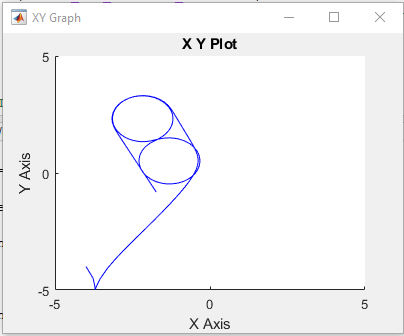
\includegraphics[width=0.5\textwidth]{imagenes/circun_desplazadas.png}
\end{figure}

Con la red neuronal se obtienen los mismos resultados, a excepción de cuando se modifica theta\_0, donde aparecen una serie de circunferencias adicionales. Se cree que es consecuencia de un sobreaprendimiento por parte de la red.
\end{document}
